\hypertarget{interface_t_p_chart_bar}{
\section{TPChartBar Class Reference}
\label{interface_t_p_chart_bar}\index{TPChartBar@{TPChartBar}}
}
{\tt \#import $<$TPChartBar.h$>$}

Inheritance diagram for TPChartBar::\begin{figure}[H]
\begin{center}
\leavevmode
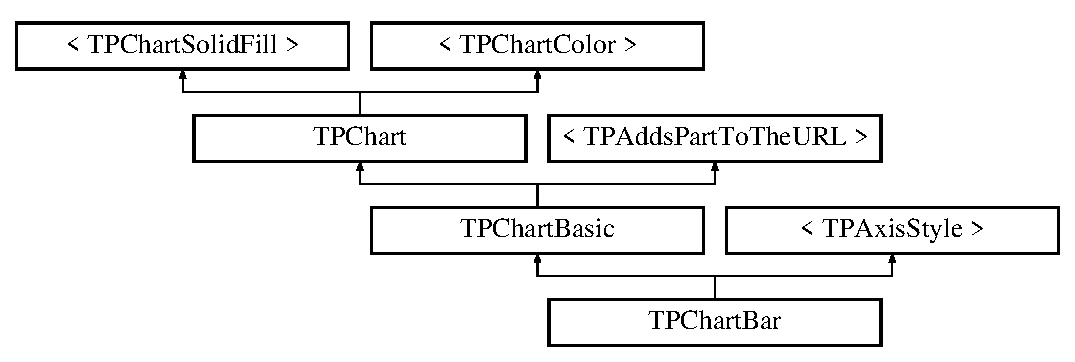
\includegraphics[height=3.31361cm]{interface_t_p_chart_bar}
\end{center}
\end{figure}
\subsection*{Properties}
\begin{CompactItemize}
\item 
TPChartTypeBar \hyperlink{interface_t_p_chart_bar_a6097d677c850f54a0e8a513356130d0}{type}
\item 
int \hyperlink{interface_t_p_chart_bar_e3b51efd638c009a91ab1b818f3dc165}{barWidth}
\item 
int \hyperlink{interface_t_p_chart_bar_8ec908b88d8db83273578b53002f654d}{spaceBetweenBars}
\item 
int \hyperlink{interface_t_p_chart_bar_2a66eac7dcb2b1f2445275af97d1955e}{spaceBetweenGroups}
\end{CompactItemize}


\subsection{Detailed Description}
Bar Chart example: \href{http://chart.apis.google.com/chart?cht=bvs&chs=200x125&chd=t:10,50,60,80,40}{\tt http://chart.apis.google.com/chart?cht=bvs\&chs=200x125\&chd=t:10,50,60,80,40}$|$50,60,100,40,20\&chco=4d89f9,c6d9fd\&chbh=20\&chds=0,160 

\subsection{Property Documentation}
\hypertarget{interface_t_p_chart_bar_e3b51efd638c009a91ab1b818f3dc165}{
\index{TPChartBar@{TPChartBar}!barWidth@{barWidth}}
\index{barWidth@{barWidth}!TPChartBar@{TPChartBar}}
\subsubsection[{barWidth}]{\setlength{\rightskip}{0pt plus 5cm}- (int) barWidth\hspace{0.3cm}{\tt  \mbox{[}read, write, assign\mbox{]}}}}
\label{interface_t_p_chart_bar_e3b51efd638c009a91ab1b818f3dc165}


Width of the bars in px 0 = automatic \hypertarget{interface_t_p_chart_bar_8ec908b88d8db83273578b53002f654d}{
\index{TPChartBar@{TPChartBar}!spaceBetweenBars@{spaceBetweenBars}}
\index{spaceBetweenBars@{spaceBetweenBars}!TPChartBar@{TPChartBar}}
\subsubsection[{spaceBetweenBars}]{\setlength{\rightskip}{0pt plus 5cm}- (int) spaceBetweenBars\hspace{0.3cm}{\tt  \mbox{[}read, write, assign\mbox{]}}}}
\label{interface_t_p_chart_bar_8ec908b88d8db83273578b53002f654d}


Width of the bars in pixel 0 = otomatic \hypertarget{interface_t_p_chart_bar_2a66eac7dcb2b1f2445275af97d1955e}{
\index{TPChartBar@{TPChartBar}!spaceBetweenGroups@{spaceBetweenGroups}}
\index{spaceBetweenGroups@{spaceBetweenGroups}!TPChartBar@{TPChartBar}}
\subsubsection[{spaceBetweenGroups}]{\setlength{\rightskip}{0pt plus 5cm}- (int) spaceBetweenGroups\hspace{0.3cm}{\tt  \mbox{[}read, write, assign\mbox{]}}}}
\label{interface_t_p_chart_bar_2a66eac7dcb2b1f2445275af97d1955e}


Space between the bars 0 = automatic \hypertarget{interface_t_p_chart_bar_a6097d677c850f54a0e8a513356130d0}{
\index{TPChartBar@{TPChartBar}!type@{type}}
\index{type@{type}!TPChartBar@{TPChartBar}}
\subsubsection[{type}]{\setlength{\rightskip}{0pt plus 5cm}- (TPChartTypeBar) type\hspace{0.3cm}{\tt  \mbox{[}read, write, assign\mbox{]}}}}
\label{interface_t_p_chart_bar_a6097d677c850f54a0e8a513356130d0}


Type of the chart One of: TPChartTypeBarBHS, TPChartTypeBarBVS, TPChartTypeBarBHG or TPChartTypeBarBVG 

The documentation for this class was generated from the following file:\begin{CompactItemize}
\item 
TPChartBar.h\end{CompactItemize}
